%!TEX root = thesis.tex
\chapter{Demonstrator}
\label{sec:demo}

\section{Stewart Platform}
The Stewart platform was introduced by D. Stewart in 1965 \citep{Ste65} and
gained popular resarch interest in robotics \citep{Szu13}, concerning
kinematics, dynamics or work space estimations. However, outside the
scientific community the Stewart platform was not widely adopted and most
designs are constrained to applications requiring \ac{6DoF}, for instance
flight simulators or \ac{CNC} machining centers. Although a Stewart platform
provides many potential advantages , sophisticated synthesis and simulation
tools are missing \citep{Ji96}. Against the background of increasing
computational capabilities and more efficient \ac{CAD} tools, this situation
might change in the future. In the scope of this thesis, the Stewart platform
promises to be a sophisticated development platform, involving computationally
expensive calculations for its kinematics and additional I/O capabilities.
Therefore, it seems to be a suitable demonstrator for a modern \acp{PAC}.

The following sections introduce the architecture of the Stewart platform in
general and the variant used in this thesis, specifying the used notation and
solving the inverse kinematics problem.

\subsection{Architecture}
While Stewart introduced the general idea of a Stewart platform in his work in
1965 \citep{Ste65}, a strict definition is missing in the literature. The only
commonality is the characterization as a parallel manipulator \citep{Szu13}
consisting out of a bottom base and an upper platform. Compared to a serial
manipulator, it consists out of multiple serial chains controlled
simultaneously and connected to a single end-effector. While this design
provides unique benefits like high accuracy, better load-to-weight ratios and
improved rigidity, it limits the available work space and causes highly
nonlinear behavior.

%\begin{figure}
%	\centering
%	\begin{subfigure}{0.3\textwidth}
%		\centering
%		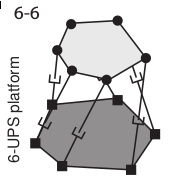
\includegraphics[width=\textwidth]{../figures/stewart_architectures_c}
%		\caption{6-UPS}
%		\label{fig:stewart_architectures_a}
%	\end{subfigure}
%	\begin{subfigure}{0.3\textwidth}
%		\centering
%		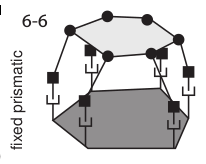
\includegraphics[width=\textwidth]{../figures/stewart_architectures_d}
%		\caption{Fixed prismatic}
%		\label{fig:stewart_architectures_b}
%	\end{subfigure}
%	\begin{subfigure}{0.3\textwidth}
%		\centering
%		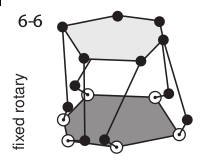
\includegraphics[width=\textwidth]{../figures/stewart_architectures_e}
%		\caption{Fixed rotary}
%		\label{fig:stewart_architectures_c}
%	\end{subfigure}
%	\caption{Different variants of Stewart platforms \citep[adopted from][]{Szu13}}
%	\label{fig:stewart_architectures}
%\end{figure}
The different variant of a Stewart platform vary in the type of the
connections and actuators, as well as their spacial configuration, i.e. the
positioning of the different connections. The most common realization utilizes
six prismatic actuator, for example hydraulic pistons or linear motors. It is
often referred to as Hexapod and associated with the term Stewart platform,
not least because of its similarity to the original design proposed by
Stewart. Other architectures utilize fixed prismatic or rotary actuators as to
vary the length of the six legs. All of these variants have its unique
benefits and drawbacks. Since the actuators in the latter design can be
realizing as commonly available servo motors, it gained popularity, especially
for low-cost designs and first prototypes. Therefore, this thesis focuses on a
servo-based architecture as shown in figure
\ref{fig:stewart}. The mechanical design and construction was not focused in
this thesis, but reused from a previous work.
\begin{figure}[tb]
	\centering
	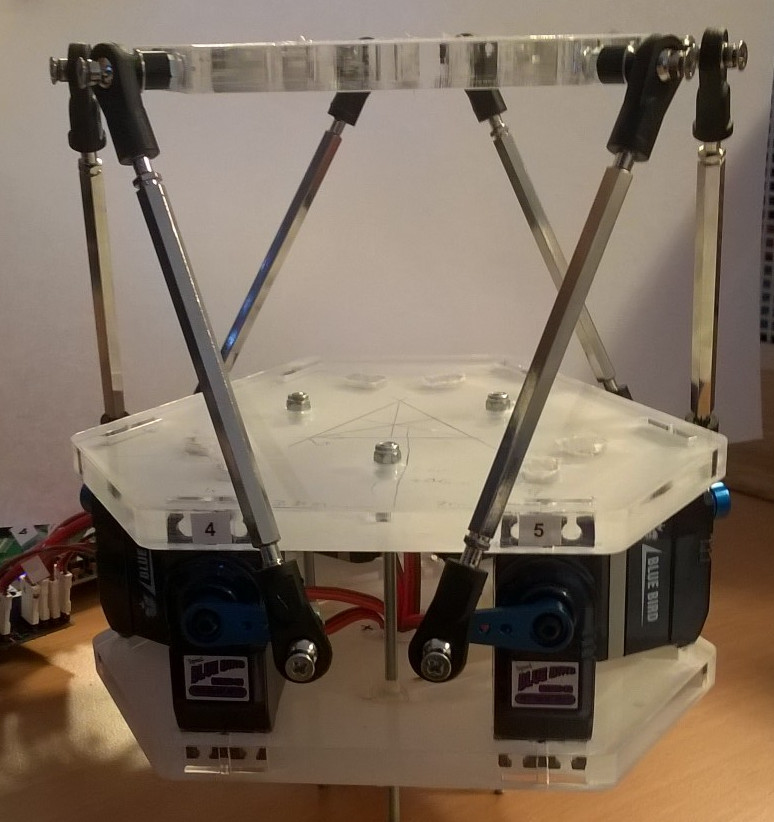
\includegraphics[width=6cm]{../figures/stewart}
	\caption{Construction of the Stewart platform prototype}
	\label{fig:stewart}
\end{figure}

\subsection{Construction and Notation}
This section introduces the basic notations, coordinate systems and dimensions
of the Steward platform used in this thesis. Consider figure
\ref{fig:stewart_notation}, showing different views annotated with relevant
notations.
\begin{figure}
	\centering
	\begin{subfigure}{0.49\textwidth}
		\centering
		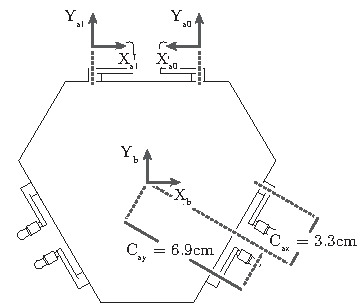
\includegraphics{../figures/stewart_base}
		\caption{Top view of base}
		\label{fig:stewart_base}
	\end{subfigure}
	\begin{subfigure}{0.49\textwidth}
		\centering
		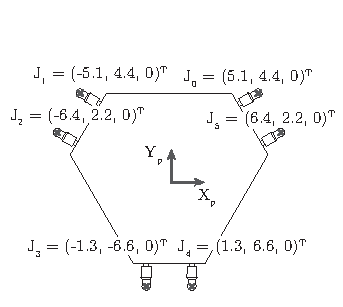
\includegraphics{../figures/stewart_platform}
		\caption{Top view of platform}
		\label{fig:stewart_platform}
	\end{subfigure}
	\par\bigskip
	\begin{subfigure}{0.49\textwidth}
		\centering
		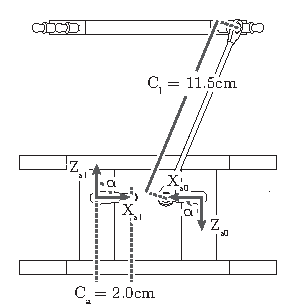
\includegraphics{../figures/stewart_side}
		\caption{Side view}
		\label{fig:stewart_side}
	\end{subfigure}
	\caption{Notations for the Stewart platform}
	\label{fig:stewart_notation}
\end{figure}

As already described previously, the system consists out of a lower base and
an upper platform, connected by six legs. For both, the base and platform, a
particular coordinate system is introduced as shown in figures
\ref{fig:stewart_base} and \ref{fig:stewart_platform}. While origin of the
base coordinate system $B$ is located in the center of the base and at the
same height as the shaft of the servos, the origin of platform's coordinate
system $P$ is located exactly above at the height of the platform joints
$J_i$. With regard to the platform's coordinate system, the coordinates of the
six joints are annotated in figure \ref{fig:stewart_platform}.

Additionally, each servo specifies its own coordinate system $S_i$, located at
the intersection point of the servo's shaft and the servo's joint position.
Thereby, the y axis points away from the base and the x axis to servo's joint
in neutral position. Resulting from these two axes, the z axis points up or
down, depending of the servo, i.e. for even servos it points down and for odd
servos it point up. Figure \ref{fig:stewart_side} illustrates the servo
coordinate systems again and showing the angle $\alpha$ of the servo arm. The
different coordinate systems for even and odd servos allow to handle all
servos analogously and respects the physical configuration of the servo arms.

Calculating the inverse kinematics of the platform requires to transform the
joints of the platform to the corresponding servo coordinate system. This is
done in two steps, by transforming them to $B$, and finally to $S_i$. While
the transformation to the base coordinate system $B$ is trivial, by simply
adding an offset $C_h$ to the z coordinate, transforming the resulting point
to the servo coordinate system $S_i$ requires more sophisticated calculations,
including rotation and scaling. At first, the base coordinate system is
rotated to match the y axis of the appropriate servo coordinate system,
followed by mirroring the x and z axis to fit the desired orientations.
Finally, the origin is translated to match the servo positions by adding and
subtracting $C_{sx}$ and $C_{sy}$ to the x and y coordinates, respectively.

\subsection{Inverse Kinematics}